\section{PS3b: N-Body Simulation}\label{sec:ps3b}

\subsection{Discussion}\label{sec:ps3b:disc}

This projects read a text file and register it to the classes and bring the files it needs and display on the window. Also, it calculates the numbers from the text and move the planets. 
I used leapfrog method to get acceleration, velocity and position for each planets. This was not hard because for accelaration I just have to devide force by mass and for velocity and position I have to multiply time.

\begin{figure}[tbh]
	\centering
	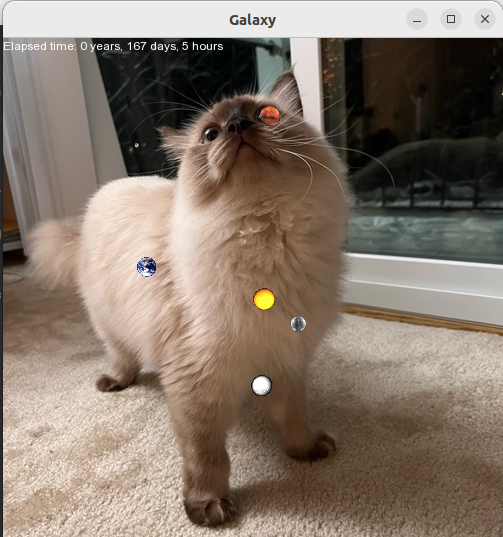
\includegraphics[width=8cm]{ps3b}
	\caption{The program shows the planets in different positions}
	\label{fig:ps3b}
\end{figure}

\subsection{Places to get help}
I got help from: SFML website, stackoverflow, c++.com, lecture slide: physics, smart-ptr

%\subsection{What I accomplished}\label{sec:ps0:accomplish}

%\subsection{What I already knew}\label{sec:ps0:knew}

%\subsection{What I learned}\label{sec:ps0:learned}

\subsection{Challenges}\label{sec:ps3b:challenges}

I tried to use the unique pointer, but I could not make it work because push back did not work, so I ended up using shared pointer since push back worked like a normal vector.
At first, in order to get force, sun is fixed argument and the planets have to be other arugments, then it moved the planets to the right. Therefore, I tried with all the planets and it worked properly.
I made a lot of mutator and accessor function since member variables are private.

\subsection{Mistakes}\label{sec:ps3b:Mistakes}

I got 2.5 points off and 10 percent. Since the program does not stop when it should, Newton's third law is not applied to my calculation, and vector for planets are not in private field. Also, about the 10 percent off, I turned the project in late for a day. 

\subsection{Extra Credit}\label{sec:ps3b:Extra Credit}

I got 0.5 extra credits because I put the clock on the left top corner with units.

\subsection{Codebase}\label{sec:ps3b:code}

Makefile
\lstinputlisting[language=Make]{ps3b/Makefile}
main.cpp
\lstinputlisting{ps3b/main.cpp}
universe.hpp
\lstinputlisting{ps3b/universe.hpp}
universe.cpp
\lstinputlisting{ps3b/universe.cpp}
CelestialBody.hpp
\lstinputlisting{ps3b/CelestialBody.hpp}
CelestialBody.cpp
\lstinputlisting{ps3b/CelestialBody.cpp}

\newpage
